\textbf{Hypothesis (H3).} If the noise failure is a missing invariance rather than missing information
(Sec.~\ref{sec:failure}), then feeding the \emph{context} encoder noisy images while the EMA target encoder keeps the clean
image should make the evaluated encoder noise-invariant. \emph{Prediction:} with the standard clean-trained probe, accuracy
at $\sigma{=}0.15$ exceeds both the baseline and the random encoder by more than the seed std, and clean accuracy drops by
less than 1.4 points. \emph{Falsified} otherwise. \emph{Ablation:} $p{=}0$, which is bit-identical to the baseline (tested).

\textbf{Change.} After the upstream augmentation, each pretraining image is noised with probability $p{=}0.5$ with its own
$\sigma\sim U(0,0.2)$, in $[0,1]$ space, clipped and re-normalised exactly like the test noise (App.~\ref{app:diff}); the noise
uses its own seeded generator, disjoint from the test-corruption seeds. Only the context encoder sees the noisy copy; masks,
loss, targets and data order are unchanged. Parameters, step time (587\,s per 15k steps vs 556--611\,s for the baseline seeds)
and peak memory (0.33\,GB) are unchanged.

\begin{figure}[t]
\centering
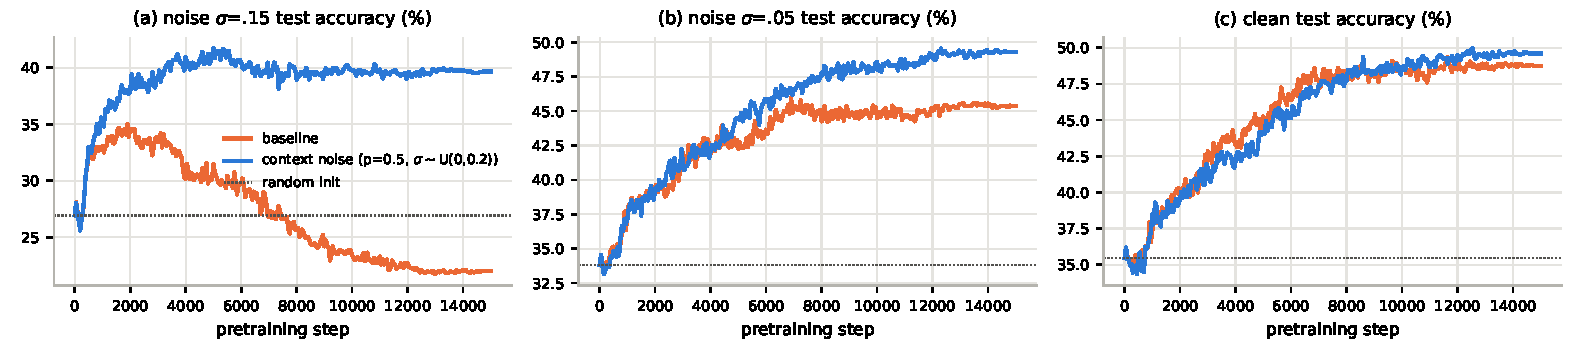
\includegraphics[width=\linewidth]{figures/fig_noise.pdf}
\caption{Test accuracy during pretraining (fixed clean-trained probe, seed 0) for the baseline and for pretraining with
noise on the context-encoder input. Dotted: the step-0 (random) encoder.}
\label{fig:noise}
\end{figure}

\begin{table}[t]\centering\small\setlength{\tabcolsep}{3.2pt}
\caption{The noise failure and two remedies (test accuracy, \%, 15k steps). Rows 3--4: the \emph{frozen} encoder (seed 0) with a \emph{mixed-trained} probe: every epoch each probe-train image is clean or, with probability $\tfrac12$, a fresh $\sigma{=}0.15$ noisy copy; $(\mathrm{lr},\mathrm{wd})$ chosen on the mean of clean and noisy validation accuracy. Row 5: pretraining with noise on the context-encoder input only ($p{=}0.5$, $\sigma\sim U(0,0.2)$), evaluated with the standard clean-trained probe; its ablation ($p{=}0$) is row 1. cos$_{.15}$: mean cosine between the clean and $\sigma{=}0.15$ features of the same test image.}
\label{tab:noise}
\begin{tabular}{lccccccc}\toprule
Encoder / probe & Clean & Occ 10\% & Occ 25\% & Occ 40\% & Noise .05 & Noise .15 & cos$_{.15}$ \\\midrule
Baseline, clean probe (5 seeds) & 48.9{\scriptsize$\pm$0.4} & 46.1{\scriptsize$\pm$0.5} & 37.3{\scriptsize$\pm$0.8} & 28.9{\scriptsize$\pm$0.4} & 45.8{\scriptsize$\pm$0.4} & 22.2{\scriptsize$\pm$1.0} & 0.71 \\
Random init, clean probe (5 seeds) & 35.1{\scriptsize$\pm$0.3} & 34.1{\scriptsize$\pm$0.9} & 29.6{\scriptsize$\pm$0.6} & 23.9{\scriptsize$\pm$0.7} & 34.2{\scriptsize$\pm$0.8} & 26.6{\scriptsize$\pm$1.3} & 1.00 \\\midrule
Baseline (s0), \emph{mixed-trained probe} & 48.8 & 46.3 & 35.8 & 27.7 & 48.1 & 39.6 & -- \\
Random init (s0), \emph{mixed-trained probe} & 34.5 & 33.3 & 28.2 & 24.1 & 34.3 & 31.3 & -- \\
\midrule
\textbf{Context-noise pretraining} (s0), clean probe & 47.5 & 46.0 & 38.4 & 29.9 & 47.6 & 41.9 & 0.95 \\
\bottomrule\end{tabular}\end{table}


\obs (Tab.~\ref{tab:noise}, Fig.~\ref{fig:noise}.) Accuracy at $\sigma{=}0.15$ rises to $\approx$41\% by step 5k and stays there
(41.9\% at 15k, +19.7 over the baseline's 5-seed mean and +15.3 over the random encoder); $\sigma{=}0.05$ improves by +1.8 and
the occlusion levels change by $-$0.1 to +1.2 (within or near seed noise). Clean accuracy is 47.5\% with the validation-selected probe ($-$1.4) and 49.6\% with
the fixed probe used for the curves (baseline seed 0: 48.8). The clean cost is therefore 1.4 points under the selected probe 
% (about 3 baseline seed standard deviations, at the edge of H3's 1.4-point tolerance) 
and none under the fixed probe: a small but probably real cost. The clean--noisy feature cosine rises from 0.71 to 0.95 while the effective rank stays high (57.7): the features are
stable \emph{and} informative. Single seed; the $\sigma{=}0.15$ gain is $\approx$20 baseline standard deviations.

\interp This is denoising~\cite{vincent2008denoising} carried out in latent space: to predict the clean target features from
a noisy context, the context encoder must map a noisy patch to (nearly) the features of its clean version, so the
noise-sensitive directions that grow during baseline training are suppressed in the evaluated encoder. Keeping the target
clean matters by design: a noisy target would ask the predictor to reproduce the noise. The I-JEPA paper deliberately avoids
hand-crafted augmentations because they bake in invariances that may not suit every task~\cite[Sec.~1]{assran2023ijepa}; our
result is the other side of that choice: without some invariance pressure, a robustness that the probe needs does not appear
by itself. \textbf{H3 is supported} on this condition. Whether the invariance generalises to corruptions not seen in
pretraining is untested (Sec.~\ref{sec:answers}).

% \textbf{Mixed probe on the noise-pretrained encoder.} The diagnostic of Sec.~\ref{sec:failure} on this encoder: the mixed-trained probe
% reaches 45.5\% at $\sigma{=}0.15$ (baseline encoder: 39.6\%) and 49.2\% clean, so only a small shift remains.
